Mein Programm erstellt neben der Ausgabe in das auf der BwInf-Seite genannte
Ausgabeformat auch einen grafischen Report im HTML-Format.
Dieser kann mit gängigen Browsern betrachtet werden.
Um Platz zu sparen, gebe ich an dieser Stelle für die BwInf-Beispiele nur die Anzahl
der gefundenen Dreicke wieder. Farbige grafische Ausgaben finden Sie im Einsendungszip.

Beispiel 3 wurde im Wettbewerbsverlauf ausgetauscht. Da mein Programm in der alten
Fassung ebenfalls 7 Dreiecke findet, gebe ich hier beide Fassungen an.

\begin{table}[h]
    \centering
    \begin{tabular}{l|lllllll}
        \textbf{Beispiel}           & 1 & 2 & 3 (alt) & 3 (neu) & 4 & 5 & 6 \\ \hline
        \textbf{gefundene Dreiecke} & 9 & 0 & 7       & 3 & 5 & 1 & 20
    \end{tabular}
    \caption{Offizielle Beispiele: gefundene Dreiecke}
    \label{tab:bwinfbeispiele}
\end{table}

Ich habe versucht, ein Beispiel mit allen möglichen Schnittpunkttypen zu konstruieren.
In diesem Beispiel findet mein Programm alle 4 Dreiecke.
Ausgaben finden Sie im Einsendungszip.

\begin{figure}[h]
\centering
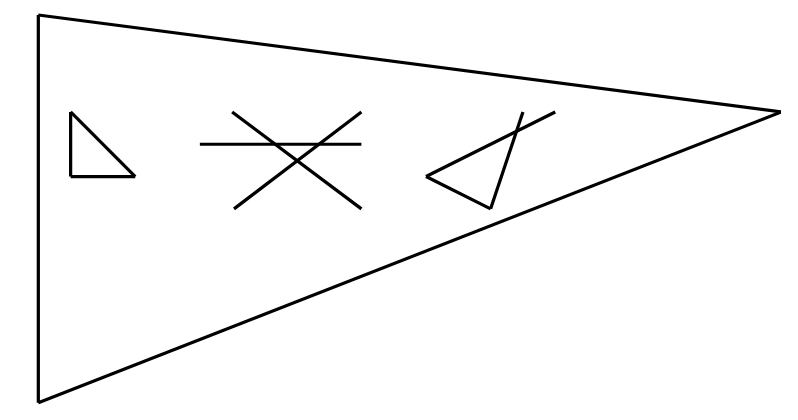
\includegraphics[width=0.7\textwidth]{eigbeispiel}
\caption{Eigenes Beispiel}
\end{figure}
